\documentclass[12pt, a4paper, oneside, justified]{article}
\usepackage{amsmath, amsthm, amssymb, graphicx}
\usepackage{geometry}
\usepackage{ragged2e} % 对齐方式
\usepackage{graphicx} % 调整大小
\usepackage[bookmarks=true, colorlinks, citecolor=blue, linkcolor=black]{hyperref}
\usepackage{ctex} % 中文支持
\usepackage{tikz} % 画图
\usepackage{listings} % 导入代码插入包
\usetikzlibrary{patterns}

\geometry{
    a4paper, % 页面尺寸
    left=3cm, % 左边距
    right=3cm, % 右边距
    top=3cm, % 上边距
    bottom=3cm, % 下边距
}

\title{KI in der Produktionstechnik}
\author{Lingjie Zhang}
\date{2024 SS}

\renewcommand{\contentsname}{Contents}

% 修改图片标签名称为 "img"
\renewcommand{\figurename}{Figure}

% 修改表格标签名称为 "table"
\renewcommand{\tablename}{Table}

% 在每个章节重置图片计数器
\counterwithin{figure}{section}

\setlength{\parskip}{1em}
\setlength{\parindent}{0pt} % 取消段落的第一行缩进

\begin{document}
\maketitle

\begin{center}
\textbf{This course is based on the lecture MW2455 of Technical University of Munich}
\end{center}

\pagenumbering{roman}
\tableofcontents
\newpage
\pagenumbering{arabic}

\section{Introduction}

\subsection{Definition of the Term Intelligence}

Natural intelligence
\par
\textbf{Intelligence} has been defined in many ways: the capacity for logic, understanding, self-awareness, 
learning, emotional knowledge, reasoning, planning, creativity, critical thinking, and problem-solving. 
More generally, it can be described as \textbf{the ability to perceive or infer information, and to retain it as knowledge to be applied towards adaptive behaviors} 
within an environment or context. Intelligence is most often studied in humans but has also been observed in both non-human animals and in plants.

The \textbf{intelligencer quotient (IQ)} is a \textbf{parameter} determined by an intelligence test 
\textbf{to evaluate intellectual performance} in general (general intelligence) or within a certain range 
(e.g, factors of intelligence) in comparison to a reference group. It always refers to a specific test, 
since there is no scientifically recognized, unambiguous definition of intelligence.

\begin{figure}[htbp]
    \centering
    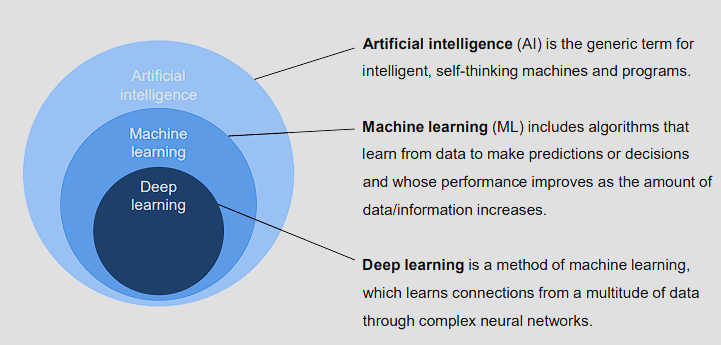
\includegraphics[scale=1]{../img/1-1.png}
    \caption{Categorization of Artificial Intelligence, Machine Learning and Deep Learning}
    \label{img/1-1}
\end{figure}

\subsection{Artificial Intelligence in Production Engineering}

\subsubsection{Machine Learning on the Different Levels of Production}

Examples of machine learning at the \href[]{https://www.mec.ed.tum.de/en/iwb/homepage/}{iwb}:
\begin{figure}[htbp]
    \centering
    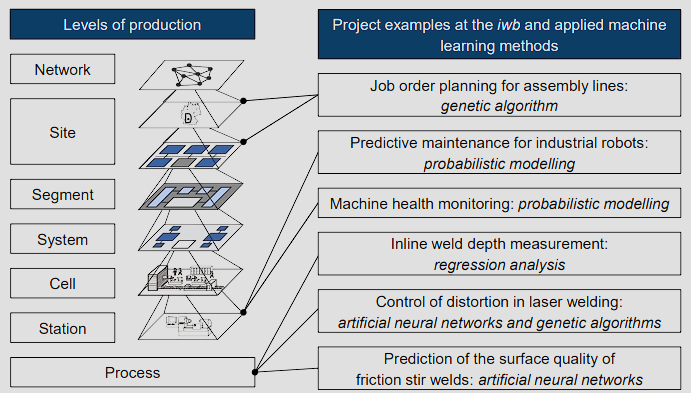
\includegraphics[scale=1]{../img/1-2.png}
    \label{img/1-2}
\end{figure}

\subsubsection{Example 1 - Job Order Planning for Assembly Lines}

\begin{figure}[htbp]
    \centering
    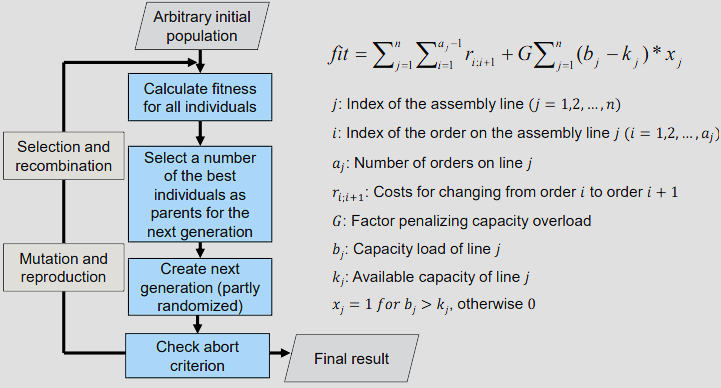
\includegraphics[scale=1]{../img/1-3.png}
    \caption{Solution: genetic algorithm}
    \label{img/1-3}
\end{figure}
\begin{figure}[htbp]
    \centering
    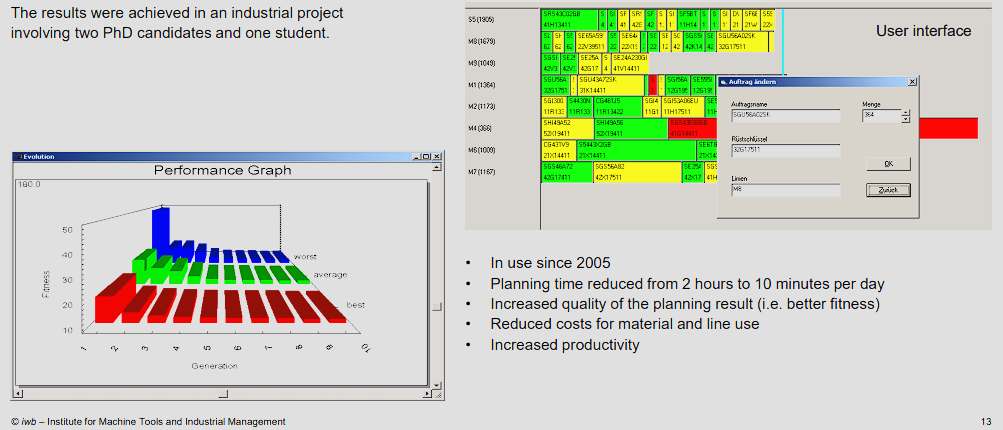
\includegraphics[scale=0.9]{../img/1-4.png}
    \label{img/1-4}
\end{figure}

\subsubsection{Example 2 - Minimization of Welding Distortions }
\vspace{1cm}

\begin{figure}[htbp]
    \centering
    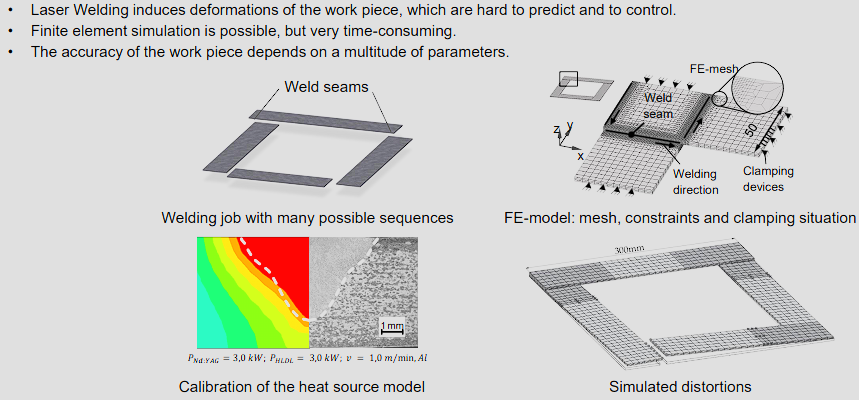
\includegraphics[scale=1]{../img/1-5.png}
    \caption{Artificial neural networks and evolutionary algorithms}
    \label{img/1-5}
\end{figure}
\begin{figure}[htbp]
    \centering
    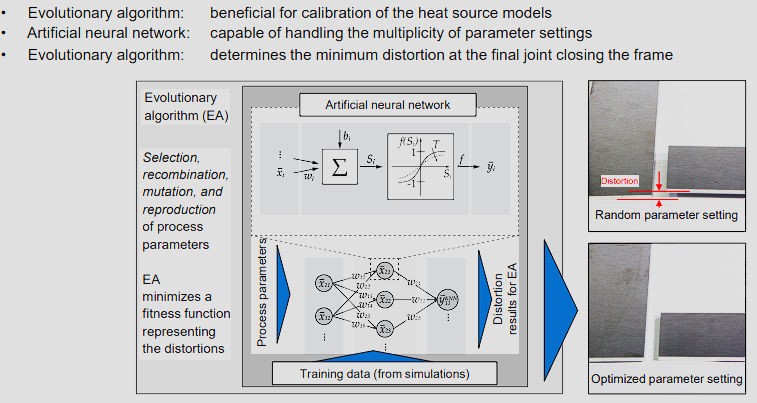
\includegraphics[scale=1]{../img/1-6.png}
    \label{img/1-6}
\end{figure}
\begin{figure}[htbp]
    \centering
    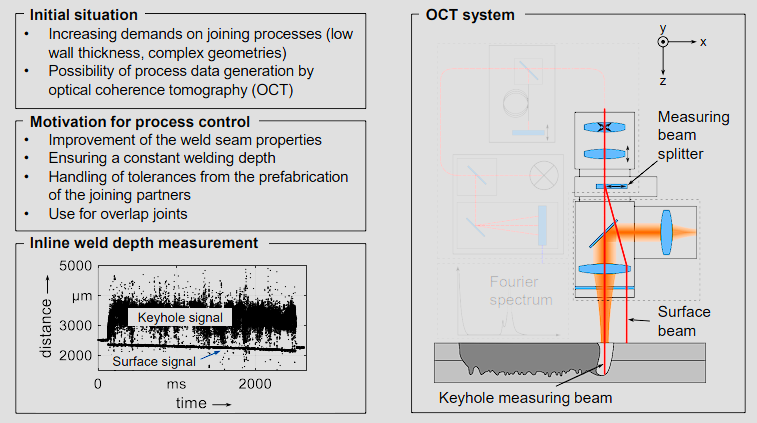
\includegraphics[scale=1]{../img/1-7.png}
    \caption{Initial situation and motivation}
    \label{img/1-7}
\end{figure}
\begin{figure}[htbp]
    \centering
    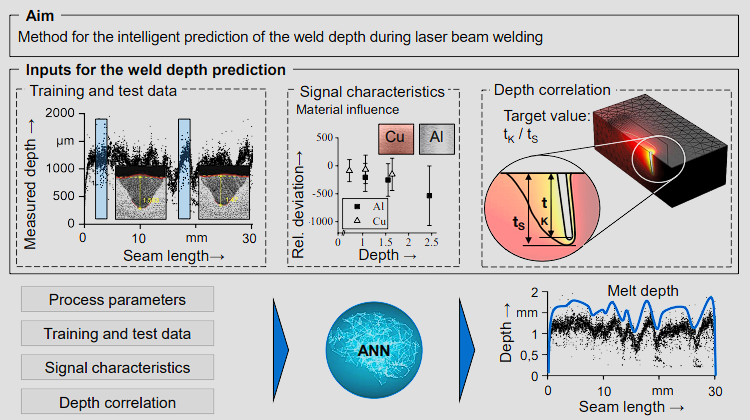
\includegraphics[scale=1]{../img/1-8.png}
    \caption{AI-based prediction of the weld depth}
    \label{img/1-8}
\end{figure}
\begin{figure}[htbp]
    \centering
    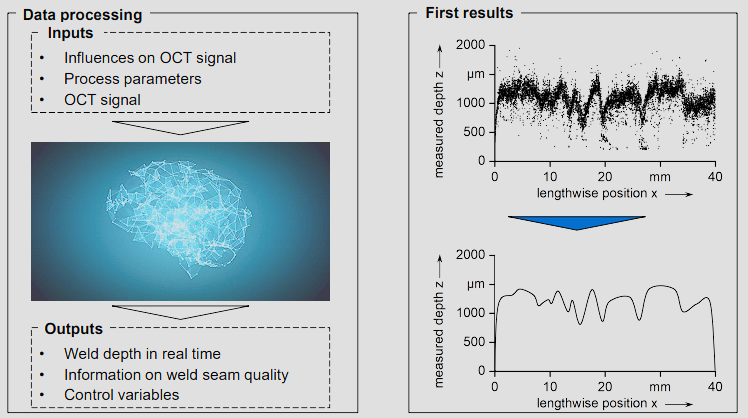
\includegraphics[scale=1]{../img/1-9.png}
    \caption{Next steps ahead}
    \label{img/}
\end{figure}

\vspace{3cm}
\subsection{Introduction to the course and to Artificial Intelligence (AI)}

\begin{table}[!h]
\centering
\begin{tabular}{c}
    MATH \& STATISTICS (Lecture) \\
    \hline
    understand and remember the basics of machine learning \\
    understand data structures, storage, preparation, features and models \\
    retrieve, compare and generalize basic methods \\
\end{tabular}
\end{table}

\begin{table}[!h]
\centering
\begin{tabular}{c}
    DOMAIN KNOWLEDGE (Lecture) \\
    \hline
    discuss applications of AI methods in production engineering \\
    challenges and approaches for the application of KDD1 in the production \\
    discuss and generalize solution concepts for industrial applications
\end{tabular}
\end{table}

\begin{table}[!h]
\centering
\begin{tabular}{c}
    PROGRAMMING \& DATABASE (Practice) \\
    \hline
    apply tools for data analysis purposes and the implementation of models \\
    apply the basic procedure to an exemplary data set \\
    identify the key challenges and derive appropriate measures to overcome them
\end{tabular}
\end{table}

\begin{table}[!h]
\centering
\begin{tabular}{c}
    COMMUNICATION \& VISUALIZATION (Group project) \\
    \hline
    translate data-driven insights into decisions and actions \\
    analyze practical problems and derive appropriate steps \\
    design concepts for knowledge acquisition from production/process data
\end{tabular}
\end{table}

\begin{figure}[!h]
    \centering
    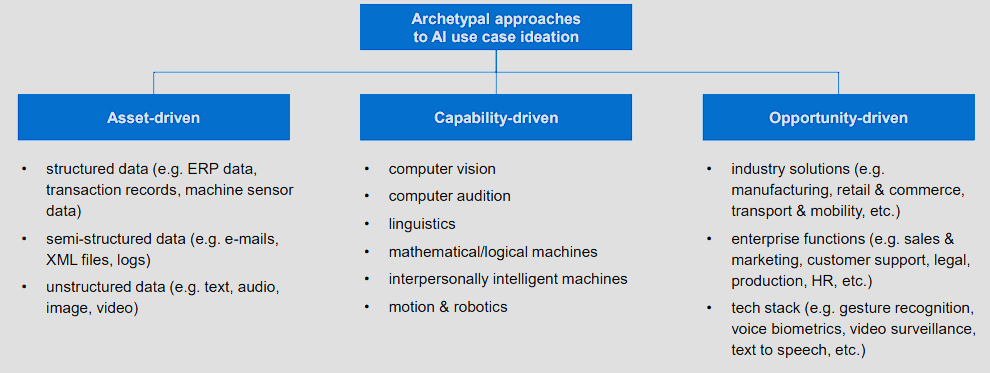
\includegraphics[scale=0.8]{../img/1-10.png}
    \caption{Application fields and opportunities of AI}
    \label{img/1-10}
\end{figure}

\begin{figure}[!h]
    \centering
    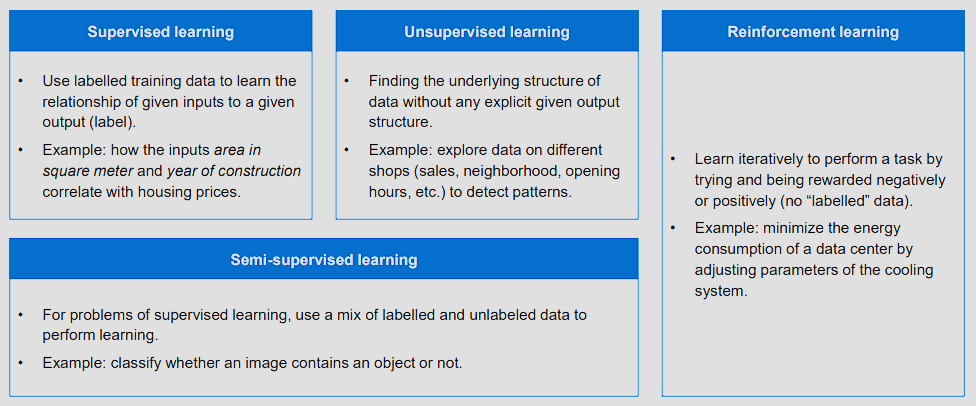
\includegraphics[scale=0.8]{../img/1-11.png}
    \caption{What is Artificial Intelligence?}
    \label{img/1-11}
\end{figure}

\vspace{2cm}
\begin{itemize}
    \item \textbf{Supervised learning} (covered in this course)
    \begin{itemize}
        \item regression
        \item classification
    \end{itemize}
    \item \textbf{Unsupervised learning} (briefly covered in this course)
    \begin{itemize}
        \item clustering
        \item data compression
    \end{itemize}
    \item \textbf{Reinforcement learning} (briefly covered in this course)
    \begin{itemize}
        \item behavior selection
        \item planning
    \end{itemize}
    \item \textbf{Evolutionary learning} (not covered in this course)
    \begin{itemize}
        \item general purpose learning
    \end{itemize}
\end{itemize}

\subsection{Recommended literature}

\begin{itemize}
    \item C.M. Bishop: Pattern recognition and machine learning. New York: Springer, 2006.
    \item T.Hastie, R. Tibshirani, und J.Friedman: The Elements of Statistical Learning. New York: Springer, 2009.
\end{itemize}

%这里
\section{Data formats and sources}
\subsection{Learning objectives}

\textbf{After participating, you will be able to…}

understand different data structures and formats and remember the respective data sources from the production environment.

\subsection{Data formats and structure}

\begin{figure}[htbp]
    \centering
    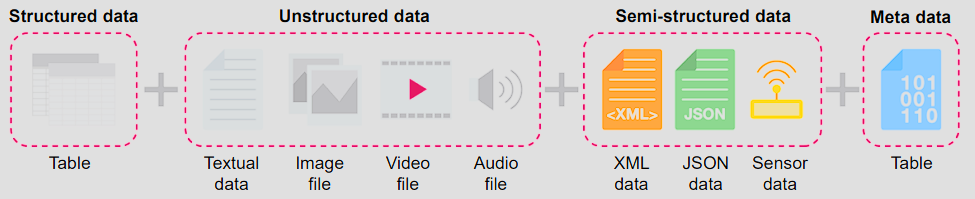
\includegraphics[scale=0.8]{../img/2-1.png}
    \label{img/2-1}
\end{figure}

\begin{table}[!h]
\centering
\begin{tabular}{p{1\textwidth}}
    Structured data \\
    \hline
    Adheres to a pre-defined model, that specifies how data can be stored, processed and accessed. \\
    Straightforward to analyze as data can be aggregated quickly from various locations. \\
    Examples: Excel files, SQL databases.
\end{tabular}
\end{table}

\begin{table}[!h]
\centering
\begin{tabular}{p{1\textwidth}}
    Unstructured data \\
    \hline
    Information that does not have a pre-defined data model or that is nor organized in a pre-defined manner. \\
    Combination of text with data such as dates, numbers and facts result in irregularities that impede a simple  processing. \\
    Examples: Audio files, video files and No-SQL databases.
\end{tabular}
\end{table}

\begin{table}[!h]
\centering
\begin{tabular}{p{1\textwidth}}
    Semi-structured data \\
    \hline
    Form of structured data that does not conform with the formal structure of data models associated with relational databases. \\
    Contains tags or other markers to separate semantic elements and enforce hierarchies of records and fields within the data. \\
    Examples: JSON data, XML data
\end{tabular}
\end{table}

\begin{table}[!h]
\centering
\begin{tabular}{p{1\textwidth}}
    Meta data \\
    \hline
    Meta data is technically not a separate form of data structure, but data about data, that provides additional information about a specific set of data. \\
    Frequently used for initial analyses in big data solutions. \\
    Examples: Location and time of a photograph
\end{tabular}
\end{table}


\subsection{Data quality}

\resizebox{\linewidth}{!}{
\begin{tabular}{|c|}
    \hline
    Data quality \\
    \hline
        \begin{tabular}{c|c|c|c}
        Intrinsic data quality & Contextual data quality & Representational data quality & Accessibility data quality \\
        \hline
        believability & value-added & interpretability & accessibility \\
        accuracy & relevancy & ease of understanding & access security \\
        objectivity & timeliness & representational consistency & \\
        reputation & completeness & concise representation & \\
        & appropriate amount of data & & \\
        \end{tabular} \\
        \hline
\end{tabular}
}

\subsection{Data sources}

\subsubsection{Architectural model of the computer-integrated production}

\begin{figure}[htbp]
    \centering
    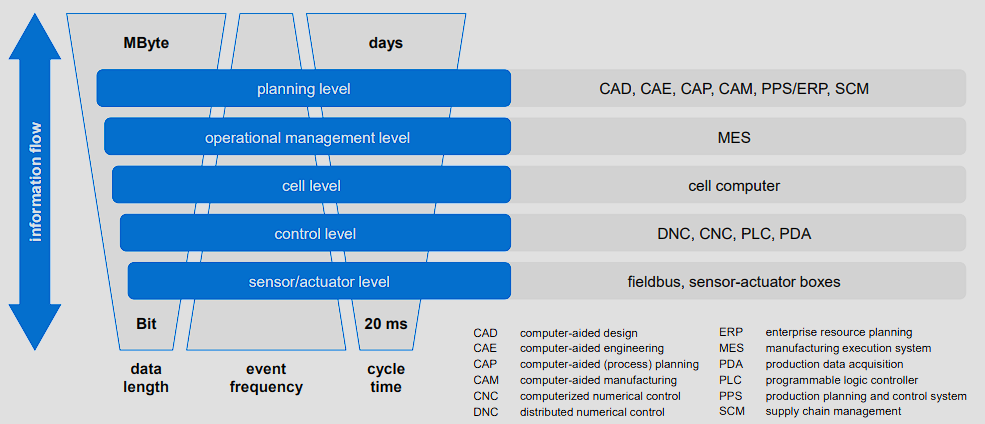
\includegraphics[scale=0.8]{../img/2-2.png}
    \label{img/2-2}
\end{figure}

\begin{figure}[htbp]
    \centering
    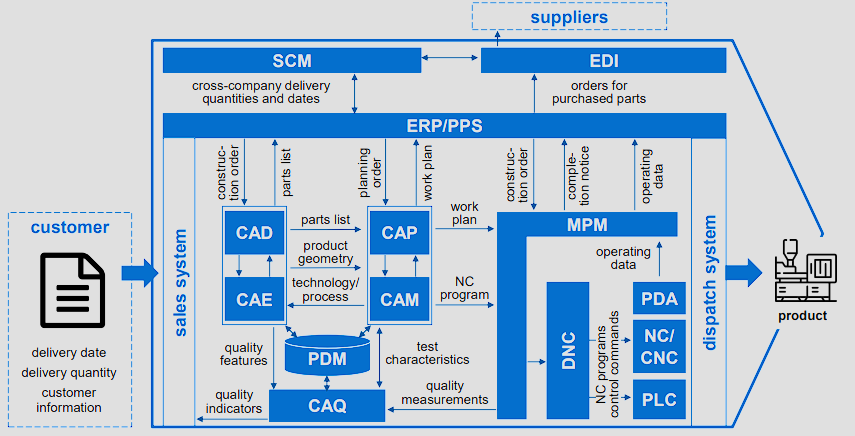
\includegraphics[scale=0.8]{../img/2-3.png}
    \label{img/2-3}
\end{figure}

\subsubsection{4.2 Information flow}

\begin{figure}[htbp]
    \centering
    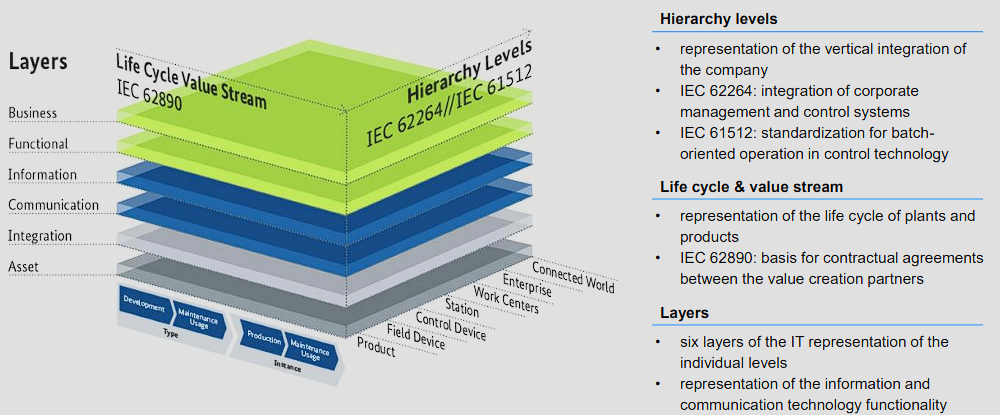
\includegraphics[scale=0.8]{../img/2-4.png}
    \caption{Information flow - Reference Architecture Model Industry 4.0 (RAMI 4.0)}
    \label{img/2-4}
\end{figure}

\textbf{Information flow - KDD process}

\begin{figure}[htbp]
    \centering
    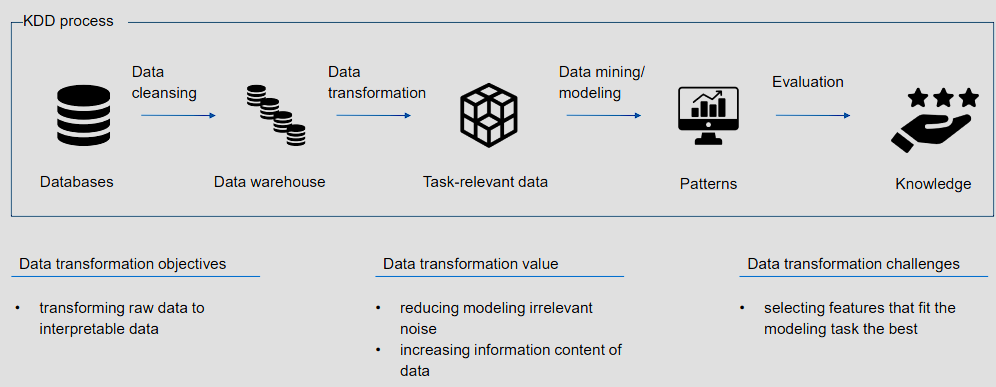
\includegraphics[scale=0.8]{../img/2-5.png}
    \caption{Information flow - KDD process}
    \label{img/2-5}
\end{figure}

\subsection{Summary}

\textbf{What you might have gathered throughout this lecture}

\begin{itemize}
    \item the characteristics of different data types and formats
    \item the dimensions of data quality
    \item representative models of production processes and architectures
    and the allocation of data sources within these models
\end{itemize}

\textbf{After a recap, you should be able to…}
\begin{itemize}
    \item understand different data structures and formats and
    remember the respective data sources from the
    production environment.
\end{itemize}

\newpage

\section{Databases and Data Cleansing}

\subsection{Knowledge Discovery in Databases (KDD)}

\begin{figure}[!h]
    \centering
    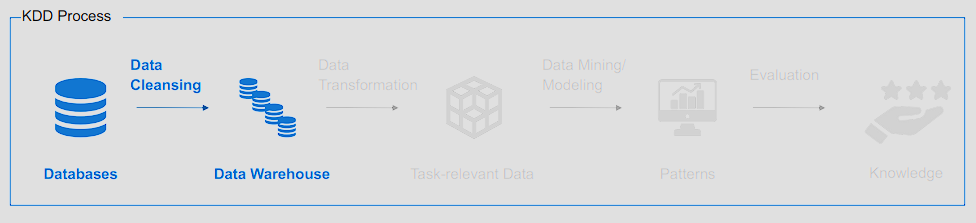
\includegraphics[scale=0.8]{../img/3-1.png}
    \caption{Overview}
    \label{img/3-1}
\end{figure}

The data passes through an operational data storage and requires cleansing to ensure the data quality before it is used in the data warehouse for reporting and analysis.

\subsection{Learning Objectives}

\textbf{Databases}

\begin{itemize}
    \item Understanding how data can be stored in databases and data warehouses
    \item Understanding the structure of different databases
    \item Processing of database queries with standardized query language (SQL)
\end{itemize}

\textbf{Data Cleansing}

\begin{itemize}
    \item Understanding the quality of data in the database
    \item Getting to know the workflow of data cleansing
    \item Understanding how data quality issues can be identified
    \item Getting familiar with the methods of data cleansing
\end{itemize}

\subsection{Databases}

Databases manage and access data efficiently.

\subsubsection{Functionality and Structure}

\begin{figure}[!h]
    \centering
    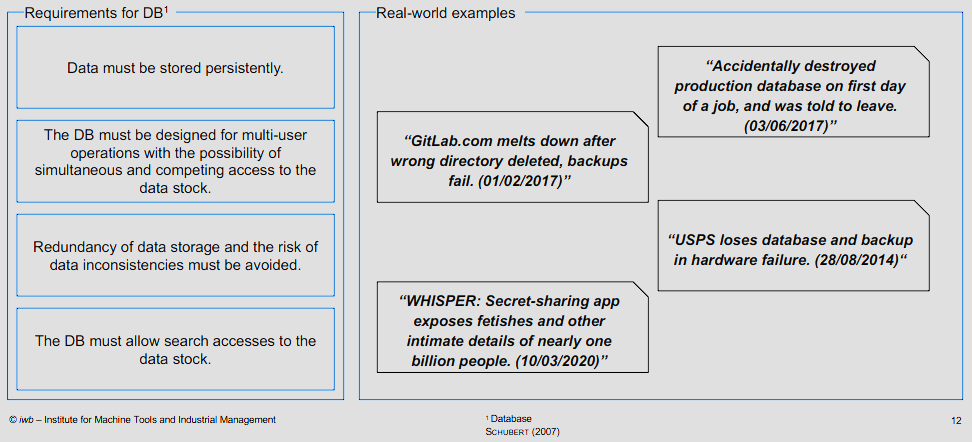
\includegraphics[width=0.8\textwidth]{../img/3-2.png}
    \label{img/3-2}
\end{figure}

\begin{figure}[!h]
    \centering
    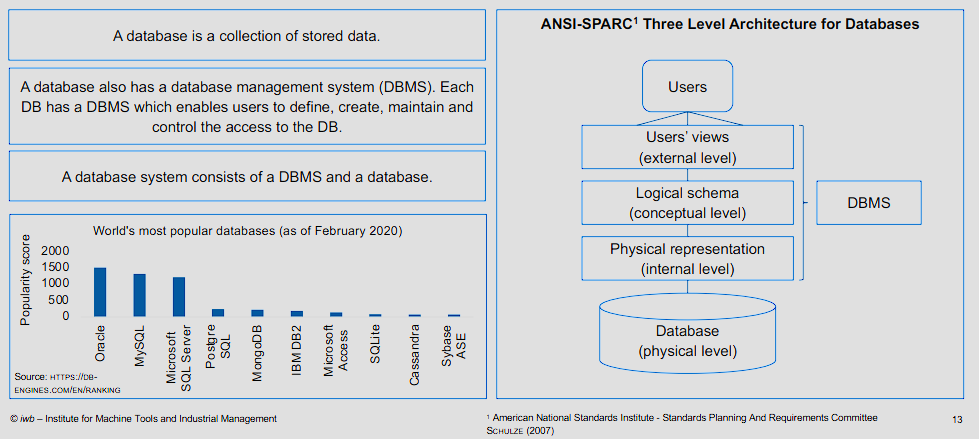
\includegraphics[width=0.8\textwidth]{../img/3-3.png}
    \label{img/3-3}
\end{figure}

\subsubsection{Database Types}

\begin{figure}[!h]
    \centering
    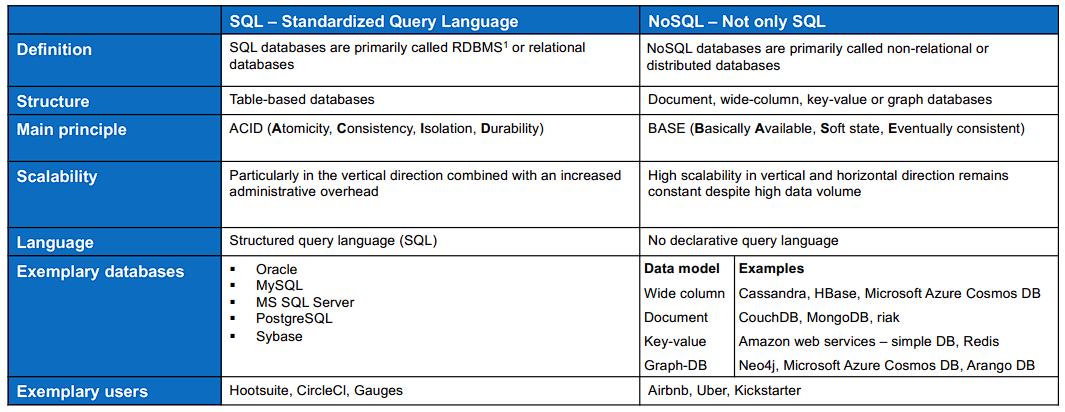
\includegraphics[width=1\textwidth]{../img/3-20.png}
    \label{img/3-20}
\end{figure}


\begin{figure}[!h]
    \centering
    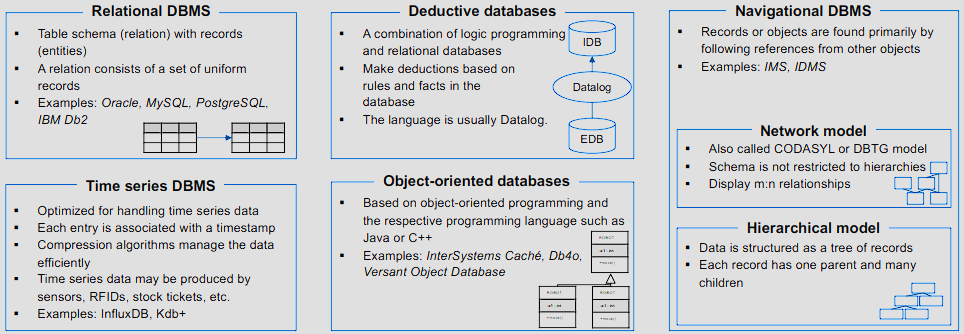
\includegraphics[width=1\textwidth]{../img/3-5.png}
    \caption{RDBMS are constantly being expanded, e.g. with object-oriented features, and are the most important DBMS.}
    \label{img/3-5}
\end{figure}

\begin{figure}[!h]
    \centering
    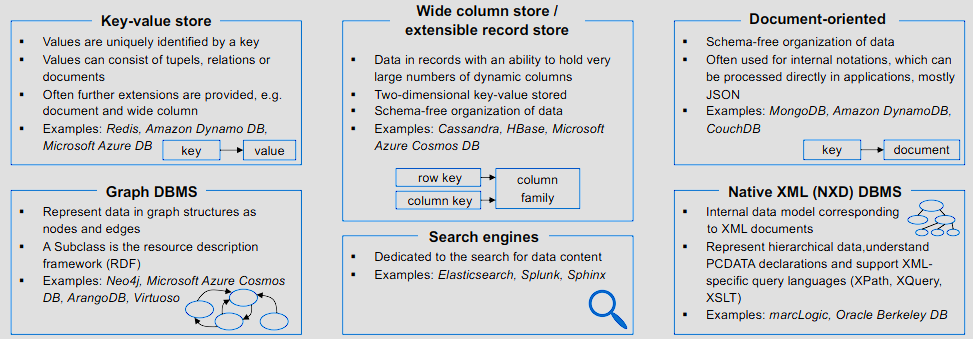
\includegraphics[width=1\textwidth]{../img/3-6.png}
    \caption{NoSQL systems gain popularity especially for Big Data applications.}
    \label{img/3-6}
\end{figure}

\begin{figure}[!h]
    \centering
    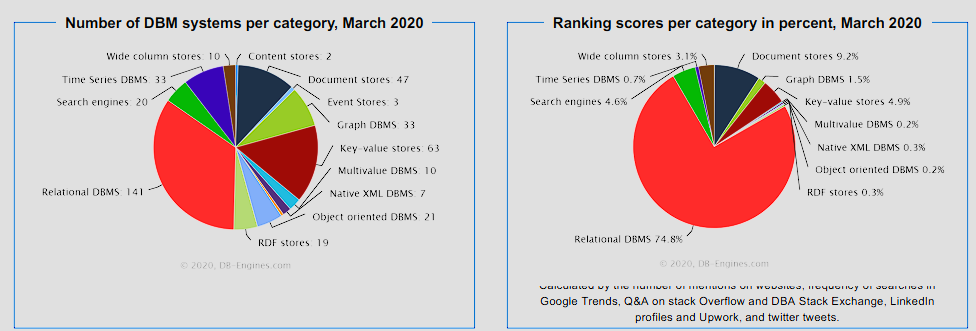
\includegraphics[width=1\textwidth]{../img/3-7.png}
    \caption{Relational DBMS dominate the market.}
    \label{img/3-7}
\end{figure}

\subsubsection{Relational Databases}

\begin{center}
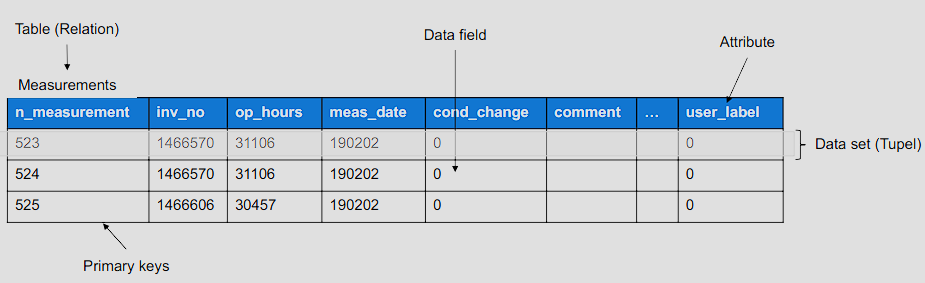
\includegraphics[width=1\textwidth]{../img/3-8.png}
\end{center}

Data is stored, changed, inserted and deleted in tables.

The logical \textbf{integrity} of a relational database is defined by the following conditions:
\begin{enumerate}
    \item Each record in a table has a unique primary key value (entity integrity).
    \item For each foreign key in the table T1. there is an identical key value in another table T2, which has been defined when T1 was created (referential integrity).
    \item The remaining constraints are fulfilled (domain integrity).
\end{enumerate}

The \textbf{primary key} is initially an attribute, or a combination of attributes of a table, that is \textbf{unique} for each record of the table.

A \textbf{foreign key} is an attribute or an attribute combination of a relation, which refers to a primary key (or key candidate) of another or the same relation.

Data integrity is a term for the assurance of the accuracy and consistency of data over its entire life-cycle.

\begin{center}
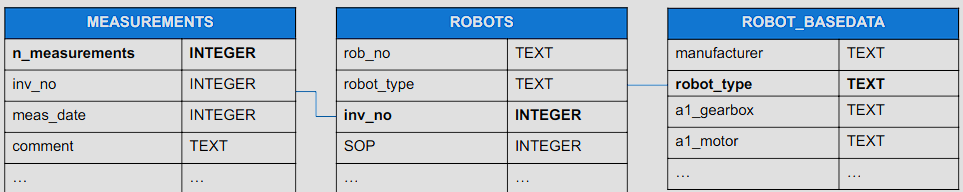
\includegraphics[width=1\textwidth]{../img/3-9.png}
\end{center}

\begin{figure}[!h]
    \centering
    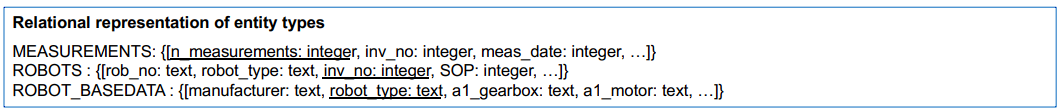
\includegraphics[width=1\textwidth]{../img/3-21}
    \label{img/3-21}
\end{figure}

A table can refer to a column of another table by using a foreign key.

\subsubsection{SQL}

\begin{center}
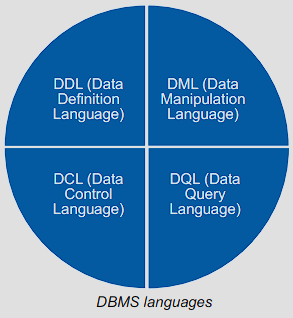
\includegraphics[width=0.3\textwidth]{../img/3-10.png}
\end{center}

\textbf{SQL = Structured Query Language}
\begin{itemize}
    \item Based on relational algebra
    \item Simple syntax
    \item Requires independence of the queries from the used DBMS.
    \item Interfaces to programming languages allow SQL commands to be transferred directly to a database system via a function call (e.g. via ODBC or JDBC).
    \item Even non-relational database systems are often equipped with an SQL-like interface.
\end{itemize}

DBMS languages are used to read, update and store data in a database and are specific to a particular data model. The dominant language is SQL.

\paragraph*{SQL: Data Definition and Manipulation Language}

\begin{center}
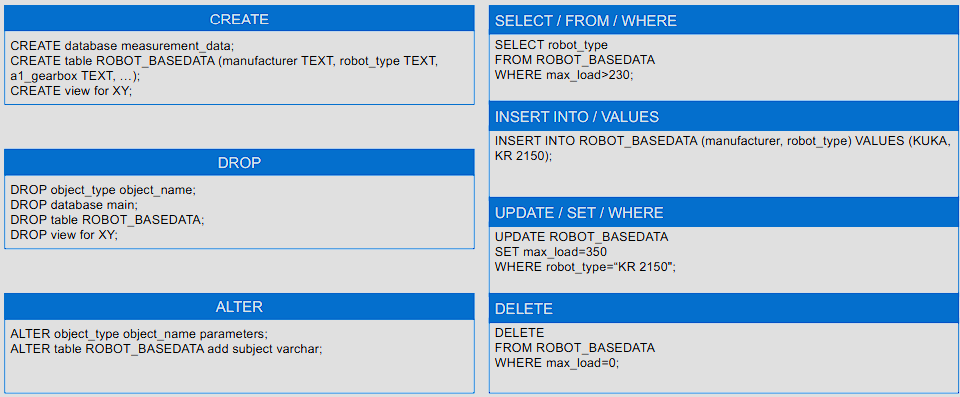
\includegraphics[width=1\textwidth]{../img/3-11.png}
\end{center}

\paragraph*{SQL: Data Query Language}

\begin{center}
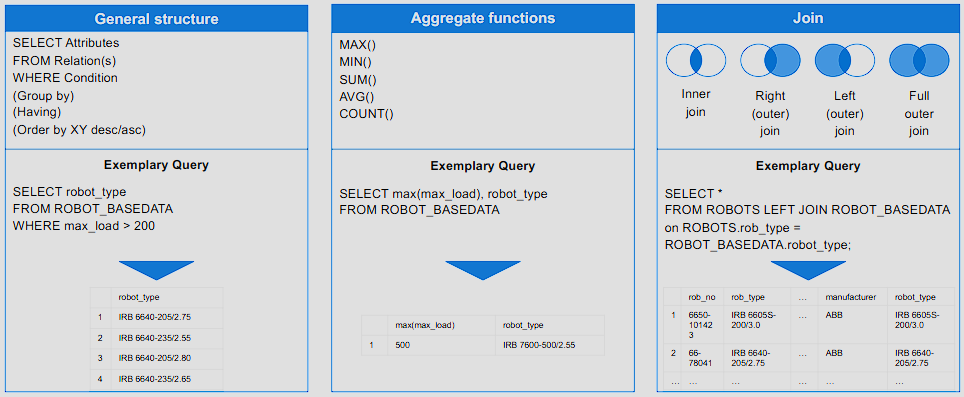
\includegraphics[width=1\textwidth]{../img/3-12.png}
\end{center}

\paragraph*{Challenges of Big Data}

\begin{center}
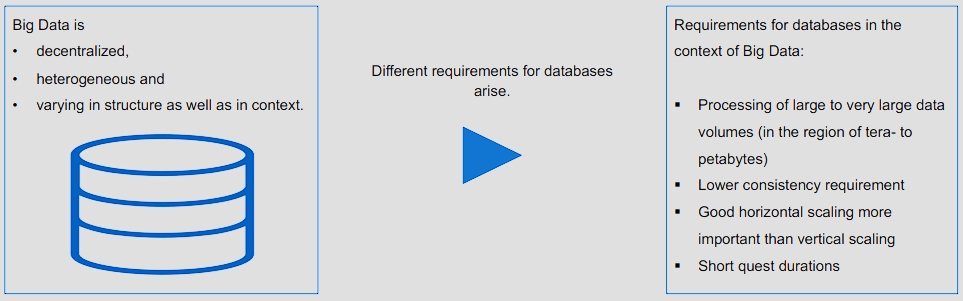
\includegraphics[width=1\textwidth]{../img/3-13.png}
\end{center}

For Big Data approaches NoSQL applications are often superior to RDBMS. However, for many database problems, the RDBMS remains the first choice.

\subsection{Data Cleansing}

Data cleansing and data integration usually accounts for 60\% and more of the total effort.

\subsubsection{Data Quality}

Data cleansing can help diminish data quality issues concerning incompleteness and incorrectness. These issues are typically caused by human errors, limitations in measurement devices and flaws in the data collection process.

\resizebox{\linewidth}{!}{
\begin{tabular}{p{8cm}|p{12cm}}
    \textbf{Measurement errors} & \textbf{Data collection errors} \\
    \hline
    \textbf{Discrepancy between the recorded value and the true value} & Apparent where \textbf{data objects or attribute values} are \textbf{omitted} or data objects are \textbf{inappropriately included} \\
    Systematic or random & Systematic or random \\
\end{tabular}
}

Given the high probability of data quality issues in real-life data, effort should be put towards detecting data quality issues and fixing those.

Data is of high quality, if it is suitable for its intended use!

\resizebox{\linewidth}{!}{
\begin{tabular}{p{10cm}|p{8cm}|p{6cm}}
\textbf{Timeliness} & \textbf{Relevance} & \textbf{Knowledge about data} \\
\hline
Dataset might only provide a snapshot of an ongoing phenomenon: If data is out of data, so are developed models and identified patterns & Available data must contain the information necessary for the application & Origin of the data must be known \\
\hline
 & Objects in available dataset must be relevant & Information on value characteristics, scale of measurements, type of features and precision must be available. \\
\hline
 & & Strongly related attributes / variables must be identified, since they are likely to provide redundant information \\
\end{tabular}
}

Data quality issues bear even higher risks for data analytics projects, as they might not be discovered until all analysis have been performed. This makes domain knowledge even more valuable for such projects.

\subsubsection{Workflow of Data Cleansing}

\begin{center}
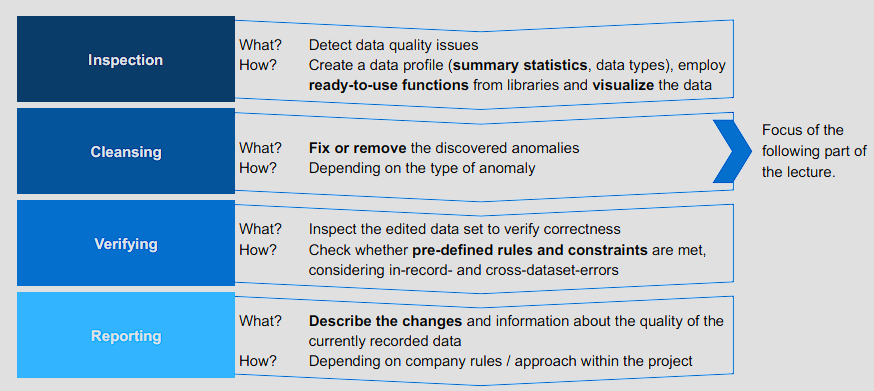
\includegraphics[width=1\textwidth]{../img/3-14.png}
\end{center}

\subsubsection{Inconsistencies and Duplicates}

\paragraph*{Inconsistent values}~{}

\underline{Description:}

Attribute values might be inconsistent, e.g. with regard to the permitted data type, categorical value or range.

\underline{Issue:}
\begin{itemize}
    \item Influence the outcome of any analysis and can ultimately lead to incorrect results
    \item Can only be identified if additional or redundant information is available
\end{itemize}

\underline{Solution:} 

\begin{enumerate}
    \item Create a data profile giving insights into the data types, missing values and generate the summary statistics
    \item Use libraries to set value constraints and to check for violation of these constraints
\end{enumerate}

\paragraph*{Duplicate data}~{}

\underline{Description:}

Duplicates are data objects that are repeated / appear more than once within a data

\underline{Issue:}

Lead to a discrepancy between the occurrence of data objects with certain characteristics in a dataset compared to the occurrence of such data objects in real life

\underline{Sloution:}

\textbf{Remove via numerous functions} in different libraries 
→ Attention should be put towards distinguishing real duplicates from \textbf{presumed duplicates}

\subsubsection{Missing Values}

\paragraph*{Reasons for missing values}~{}

\begin{itemize}
    \item Information was \textbf{not collected}
    \item Errors in manual data collection
    \item Equipment errors
    \item Measurement errors
    \item Attribute / variable \textbf{not applicable} to all objects
    \item \textbf{Non-integrable data sources}
\end{itemize}

\paragraph*{Issues caused}~{}

\begin{itemize}
    \item Loss of efficiency with regard to handling and analysis of the data
    \item Bias resulting from differences between missing and complete data
\end{itemize}

\paragraph*{Detecting and exploring missing values}~{}

\begin{itemize}
    \item Functions from different programming languages allow to detect and unify missing values.
    \item Checking the dimensions and verifying the data type
    \item Visualization of the distribution can be beneficial
\end{itemize}

It is important to assess the relevance of the missing values with regard to their frequency and their significance for further analysis.

\paragraph*{Types of missing values}~{}

\textbf{Missing Completely At Random (MCAR)}
\begin{itemize}
    \item \underline{Definition:} Missing of a value is neither related to the variable it describes nor any other variable of the data object.
    \item \underline{Example:} The sensor recording the regarded value was unavailable for that measurement.    
\end{itemize}

\textbf{Missing At Random (MAR)}
\begin{itemize}
    \item \underline{Definition:} Missing of a value is not dependent on the variable it describes, but dependent on values of one or more other variables of the data object.
    \item \underline{Example:} A measurement might not have been taken because another measurement already deemed the product a reject.    
\end{itemize}

\textbf{Not Missing At Random (NMAR)}
\begin{itemize}
    \item \underline{Definition:} Missing of a value is dependent on its hypothetical value and/or other variable's values.
    \item \underline{Example:} Elderly women are less likely to submit their age in questionnaires.    
    The type of the missing values will influence which approach of handling missing values is feasible. Thus, it is imperative to be familiar with the different types.
\end{itemize}

\begin{center}
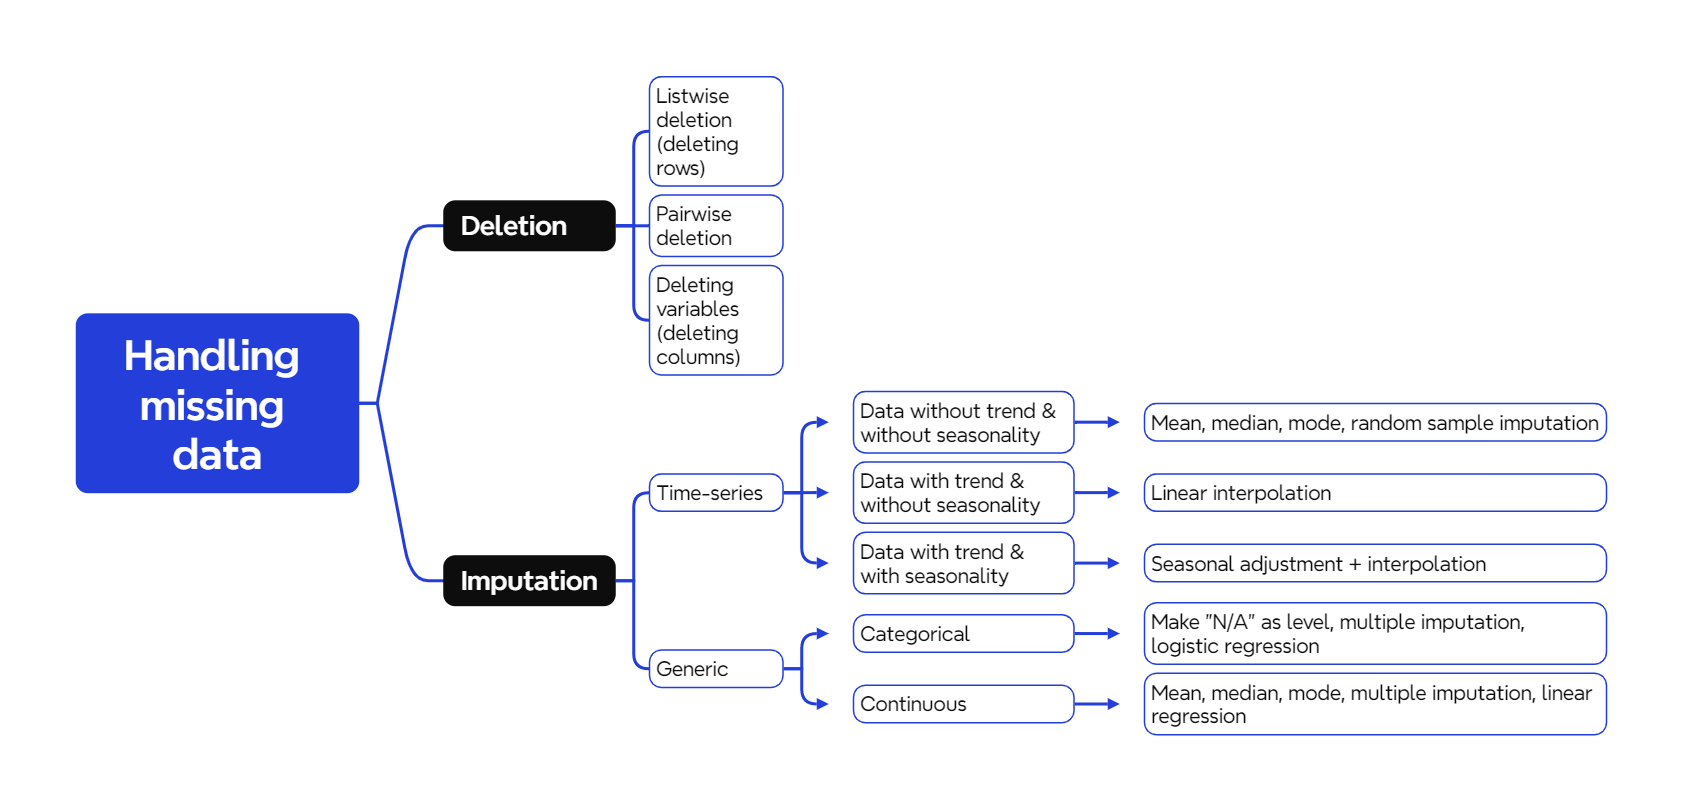
\includegraphics[width=1\textwidth]{../img/3-15.png}
\end{center}

\subsubsection{Noise}

\textbf{Description}
\begin{itemize}
    \item Random component of a measurement error
    \item Distortion of a value or addition of spurious objects
    \item Typical causes:
    \item Environmental conditions (e.g. vibrations from other machines)
    \item Deployed sensor systems
\end{itemize}

\textbf{Solution}

Applying filters to signals decreases the signal-to-noise-ratio, but can also decrease the information content.

Solutions for noise in time series:
\begin{itemize}
    \item Filters
    \item Averaging (only feasible if time-wise synchronized measurement): 
    $$
    \{ \bar{x}_m \} = \frac{1}{N} \sum _{n=1}^N\{x_m\} _k
    $$
\end{itemize}

Solutions for noise in images:
\begin{itemize}
    \item Convolution with kernels for
    \item Edge detection
    \item Sharpening
    \item Smoothing
\end{itemize}

\begin{center}
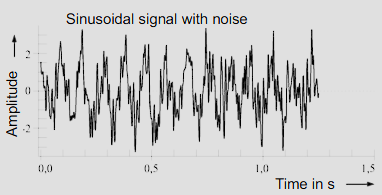
\includegraphics[width=0.4\textwidth]{../img/3-16.png}
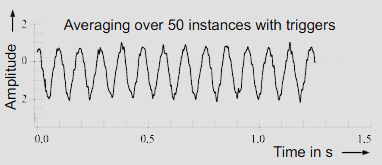
\includegraphics[width=0.5\textwidth]{../img/3-17.png}
\end{center}

\begin{center}
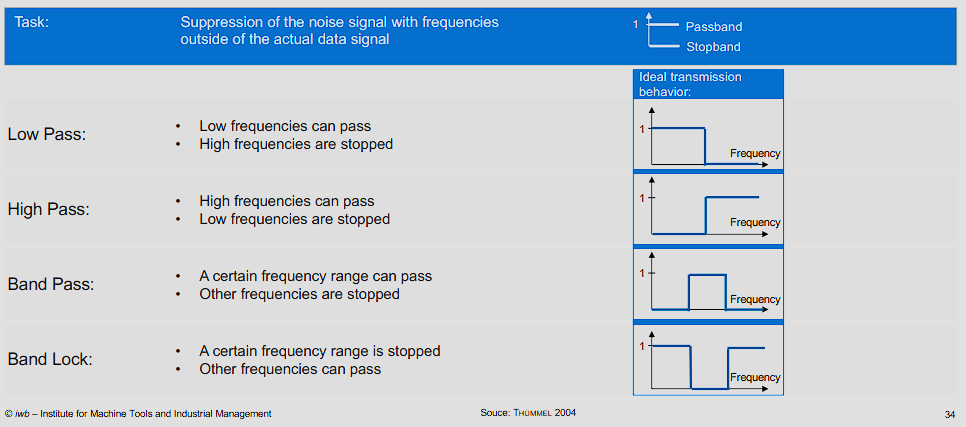
\includegraphics[width=1\textwidth]{../img/3-18.png}
\end{center}

\subsubsection{Outliers}

\paragraph*{Distinction from noise}~{}

Outliers can be valid and hold important information. 
→ e.g. for condition monitoring

\paragraph*{Types of outliers}~{}
\begin{itemize}
    \item Data object outliers differ from the other data objects in the dataset in numerous characteristics.
    \item Attribute value outliers are identified through a comparison against the distribution of the rest of the values for that attribute.    
\end{itemize}

\paragraph*{Issues caused}
\begin{itemize}
    \item Outliers can influence the data transformation outcome and thus lead to wrong conclusions in the evaluation step.
\end{itemize}

There is no precise way to define and identify outliers in general. Instead the raw observations must be interpreted as to whether a value is and outlier or not. Statistical methods can be employed to identify observations.

\underline{How to find outliers?}

\begin{figure}[!h]
    \centering
    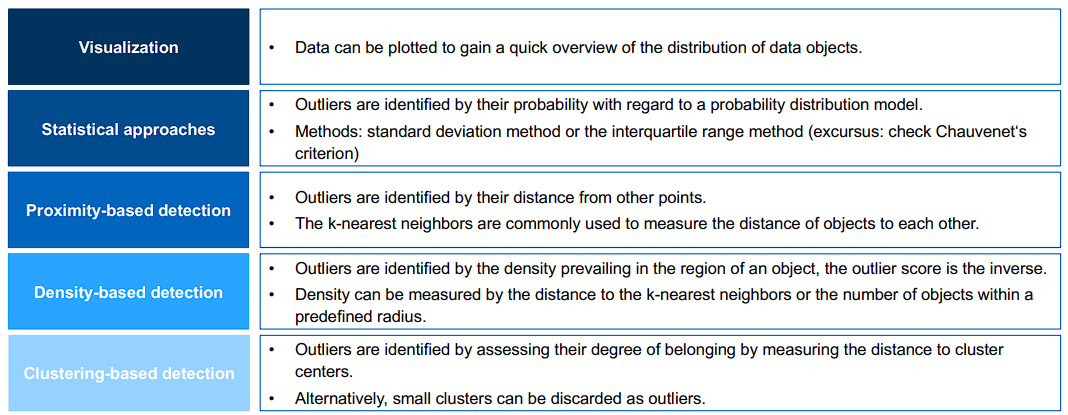
\includegraphics[width=0.8\textwidth]{../img/3-22.png}
\end{figure}

\underline{And how to solve outliers? And issues?}

\begin{figure}[!h]
    \centering
    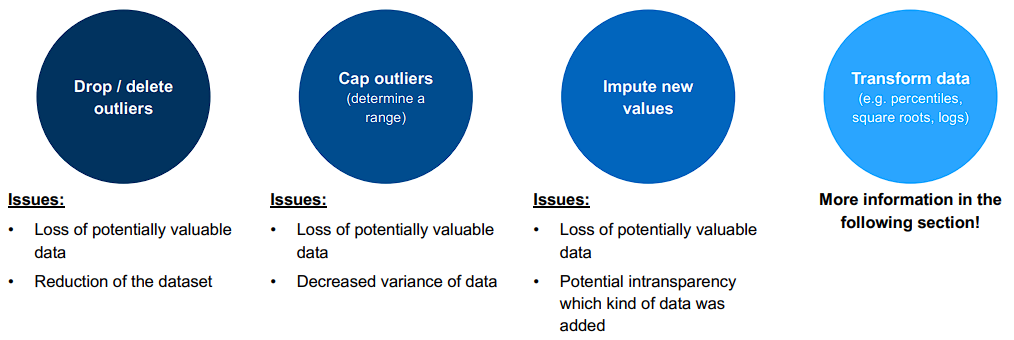
\includegraphics[width=0.8\textwidth]{../img/3-23.png}
\end{figure}
Instead of dealing with outliers explicitly, robust algorithms should be chosen wherever feasible. Even more so when working with
classification and regression algorithms.

\subsubsection{Normalization}

\paragraph*{Normalization}~{}

\underline{Description:}
\begin{itemize}
    \item Changes numeric values of different attributes / variables to a common scale, typically setting the range between 0-1
\end{itemize}

\underline{Benefits:}
\begin{itemize}
    \item Helps preventing variables with larger ranges to influence the model more heavily than those with smaller ranges.
\end{itemize}

\underline{Methods:}
\begin{itemize}
    \item Min-Max-Normalization → $x_{new}=\frac{x-x_{min}}{x_{max}-x_{min}}$
    \item Unit Vector Normalization
    \item Z-Normalization
\end{itemize}

\paragraph*{Standardization}~{}

\underline{Description:}
\begin{itemize}
    \item Assumes that a \textbf{Gaussian distribution} is present
    \item Sets the \textbf{mean of the data to 0} and the standard deviation to 1
\end{itemize}

\underline{Benefits:}
\begin{itemize}
    \item Improves the numerical stability of the model and often reduces training time
\end{itemize}

\underline{Methods:}
\begin{itemize}
    \item Z-Normalization (Standardization) $z_i=\frac{x_i-\bar x}{s}$
\end{itemize}
 
\textit{Normalization is used when trying to model relations between attributes / variables. It reduces the bias that might originate from different scales.}

\subsubsection{Transformation}

\underline{\textbf{Methods:}}

\paragraph*{Simple Functions}~{}

\underline{Description:}
\begin{itemize}
    \item Some functions can be used to reduce skewness and variance.
\end{itemize}

\underline{Methods:}
\begin{itemize}
    \item Logarithm, Square Root, Box Cox
\end{itemize}

\paragraph*{Discretization}~{}

\underline{Description}
\begin{itemize}
    \item Process of mapping continuous values to discrete values
    \item Commonly used for classification
\end{itemize}

\paragraph*{Binarization}~{}

\underline{Description:}
\begin{itemize}
    \item Maps a continuous or categorial attribute onto one or more binary variables (might increase dimensionality, e.g. one hot encoding)
    \item Commonly used for association analysis
\end{itemize}

\textit{Attribute / variable transformation maps an entire set of values of a given attribute / variable to a new set of replacement values. It allows to deal with skewness and allows for more performant computing. All methods lead to a loss of information.}

\begin{center}
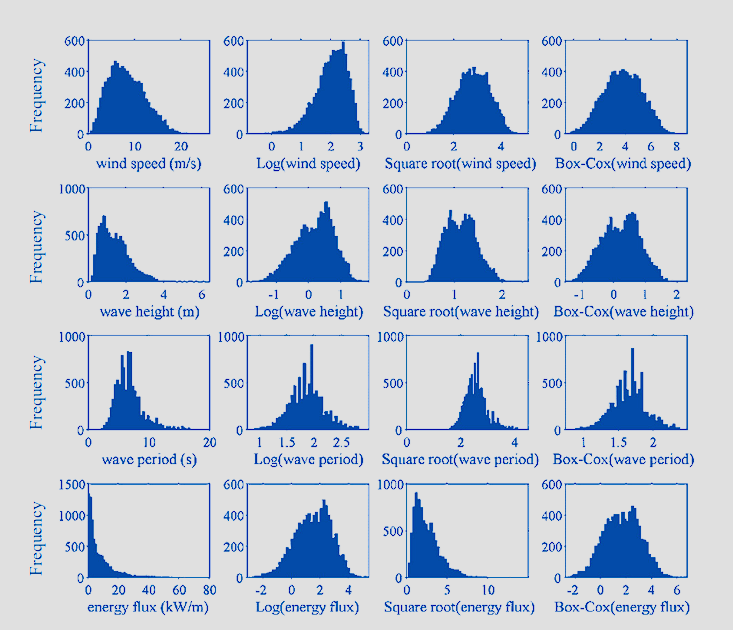
\includegraphics[width=0.8\textwidth]{../img/3-19.png}
\end{center}

\subsubsection{Highly Correlated Data}

Highly correlated data are unlikely to contribute any further information and very likely to cause overfitting. Thus, a correlation coefficient matrix should be calculated to check for possible correlations between attributes / variables. Overall, domain knowledge helps identifying cases, in which calculation the coefficient is necessary.

\textbf{Linear relationships:}

Person's Correlation Coefficient:
$$
r=\frac{cov(x,y)}{\sigma_x\cdot\sigma_y}
$$
\begin{itemize}
    \item Coefficient returns a value between -1 and 1, i.e. a full negative correlation to a full positive correlation
    \item Value of 0 means no correlation, whereas an absolute value over 0.5 indicates a notable correlation
\end{itemize}

\textbf{Non-linear relationships:}

Spearman's Correlation Coefficient:
$$
r=\frac{cov(rank(x),rank(y))}{\sigma_{rank(x)}\cdot\sigma_{rank(y)}}
$$

\begin{itemize}
    \item Non-Gaussian distribution is no issue (non-parametric correlation)
    \item Assumes a monotonic relationship
    \item Rank-based approach quantifies the association between variables using the ordinal relationship between the values rather than the specific values
\end{itemize}

\subsubsection{Dimensionality}

\paragraph*{Inconsistent dimensionality}~{}

\underline{Problem}
\begin{itemize}
    \item Machine learning \textbf{algorithms require} training and test \textbf{data of consistent dimensions}.
    \item \textbf{Data} from time series and real production applications might not fulfill this requirement.
\end{itemize}

\underline{Solution approach}
\begin{itemize}
    \item Methods presented to handle missing values / outliers
    \item Methods of the data transformation section to unify data dimensionality
\end{itemize}

\paragraph*{High dimensionality}~{}

\underline{The "Curse of Dimensionality":}
\begin{itemize}
    \item Some data analysis becomes significantly harder
    \item Data becomes increasingly sparse in the space it occupies
    \item For classification there are not enough objects to create a model that can predict all classes
    \item For clustering the density and distance are less meaningful
\end{itemize}

\subsection{Data Warehouse}

\textbf{Definition}

A data warehouse (DW) \textbf{is a central repository of integrated data optimized for analysis purposes} 
and combines data from several, usually heterogeneous sources. \textbf{Extract-transform-load (ETL) is the main 
process} to build a data warehouse system.

\textit{The decoupling of a central data warehouse from the databases supplying the data leads on the one hand to 
a relief of the operative systems and on the other hand opens the option to optimize the analysis-oriented 
system for the needs of evaluations and reports.}

\end{document}